\documentclass[aspectratio=169,12pt]{beamer}

% ======================= 中文支持 =======================
\usepackage[UTF8,heading=true,scheme=plain]{ctex}

% ======================= Beamer 主题 =======================
\usetheme{Madrid}
\usecolortheme{whale}
\setbeamertemplate{navigation symbols}{}
\setbeamertemplate{footline}[page number]
\setbeamerfont{frametitle}{size=\large,series=\bfseries}
\setbeamerfont{title}{size=\Large,series=\bfseries}

% ======================= 自定义颜色 =======================
\usepackage{xcolor}
\definecolor{tongjiBlue}{RGB}{37,99,235}
\definecolor{tongjiRed}{RGB}{220,38,38}
\definecolor{tongjiGreen}{RGB}{22,163,74}
\definecolor{tongjiGray}{RGB}{107,114,128}

\setbeamercolor{structure}{fg=tongjiBlue}
\setbeamercolor{title}{fg=white,bg=tongjiBlue}
\setbeamercolor{frametitle}{fg=tongjiBlue}

% ======================= 常用宏包 =======================
\usepackage{amsmath,amssymb}
\usepackage{graphicx}
\usepackage{booktabs}
\usepackage{array}
\usepackage{multirow}
\usepackage{tikz}
\usepackage{pifont}

\graphicspath{{../thesis/figures/}}

\newcommand{\cmark}{\textcolor{tongjiGreen}{\ding{51}}}
\newcommand{\xmark}{\textcolor{tongjiRed}{\ding{55}}}
\newcommand{\up}[1]{\textcolor{tongjiRed}{\textbf{$+$#1}}}
\newcommand{\down}[1]{\textcolor{tongjiGreen}{\textbf{$-$#1}}}

% ======================= 标题信息 =======================
\title[三路融合 ZS-CIR]{基于视觉代理与描述融合的\\零样本组合式图像检索改进}
\subtitle{本科毕业设计答辩}
\author{杨昊明}
\institute[同济大学]{同济大学 电子与信息工程学院\\计算机科学与技术专业}
\date{2026 年 5 月}

\begin{document}

% ==================== Slide 1: 封面 ====================
\begin{frame}
\titlepage
\begin{center}
\small 指导教师：（填写指导教师）
\end{center}
\end{frame}

% ==================== Slide 2: 目录 ====================
\begin{frame}{答辩提纲}
\tableofcontents[hideallsubsections]
\end{frame}

% ==================== Part 1: 研究背景 ====================
\section{研究背景与问题}

\begin{frame}{\S1~组合式图像检索任务}
\begin{columns}[T]
\begin{column}{0.55\textwidth}
\textbf{任务形式}：给定一张\textbf{参考图像} $I_r$ 和一段\textbf{修改文本} $t$，在图库 $\mathcal{G}$ 中检索符合修改意图的目标图像。

\vspace{0.8em}
\textbf{典型场景}：
\begin{itemize}\small
  \item 服饰检索：``同款但颜色改为红色的裙子''
  \item 场景检索：``保留原场景，把猫换成狗''
\end{itemize}

\vspace{0.8em}
\textbf{零样本设定（ZS-CIR）}：
\begin{itemize}\small
  \item 不依赖目标数据集训练
  \item 仅依靠预训练模型泛化
  \item 更贴近真实应用
\end{itemize}
\end{column}
\begin{column}{0.42\textwidth}
\centering
\begin{tikzpicture}[scale=0.7, every node/.style={transform shape}]
\node[draw=tongjiBlue, thick, rounded corners, fill=blue!5, minimum width=2.5cm, minimum height=1.2cm] (ref) at (0,2) {参考图 $I_r$};
\node[draw=tongjiBlue, thick, rounded corners, fill=blue!5, minimum width=2.5cm, minimum height=1.2cm] (text) at (0,0) {修改文本 $t$};
\node[draw=tongjiRed, thick, rounded corners, fill=red!5, minimum width=2cm, minimum height=1.5cm] (model) at (3.5,1) {\small 检索模型};
\node[draw=tongjiGreen, thick, rounded corners, fill=green!5, minimum width=2.5cm, minimum height=1.2cm] (tgt) at (7,1) {目标图 $I_t$};
\draw[->, thick] (ref) -- (model);
\draw[->, thick] (text) -- (model);
\draw[->, thick] (model) -- (tgt);
\node at (3.5, 2.5) {\small 图库 $\mathcal{G}$};
\end{tikzpicture}
\end{column}
\end{columns}
\end{frame}

\begin{frame}[shrink=10]{\S1~OSrCIR基线方法及其局限}
\textbf{OSrCIR (CVPR 2025 Highlight)}：首个单阶段反思推理的零样本组合检索方法
\begin{center}
\begin{tikzpicture}[scale=0.68, every node/.style={transform shape, font=\scriptsize}]
\node[draw, rounded corners, fill=blue!10, minimum width=2cm, minimum height=0.7cm] (input) at (0,0) {参考图+文本};
\node[draw, rounded corners, fill=orange!10, minimum width=2cm, minimum height=0.7cm] (mllm) at (3,0) {MLLM推理};
\node[draw, rounded corners, fill=green!10, minimum width=2cm, minimum height=0.7cm] (d1) at (6,0) {目标描述 $D_1$};
\node[draw, rounded corners, fill=purple!10, minimum width=1.8cm, minimum height=0.7cm] (clip) at (9,0) {CLIP};
\node[draw, rounded corners, fill=red!10, minimum width=1.8cm, minimum height=0.7cm] (ret) at (12,0) {检索结果};
\draw[->, thick] (input) -- (mllm);
\draw[->, thick] (mllm) -- (d1);
\draw[->, thick] (d1) -- (clip);
\draw[->, thick] (clip) -- (ret);
\end{tikzpicture}
\end{center}

\vspace{0.3em}
\textbf{三个关键问题}：
\begin{itemize}\footnotesize
  \item[\xmark] \textbf{缺乏视觉验证}：只调用一次 MLLM，若描述偏差则无法纠正
  \item[\xmark] \textbf{单一路径脆弱}：CLIP 对文本敏感，检索全部依赖一条描述
  \item[\xmark] \textbf{难以利用 AI 生成图像}：直接使用会引入幻觉反而退化
\end{itemize}

\vspace{0.3em}
\begin{block}{\footnotesize 核心研究问题}
\footnotesize 如何将 AI 生成图像作为\textbf{``可用但不可信''}的辅助信号纳入检索流程，同时避免其成为新的误差来源？
\end{block}
\end{frame}

% ==================== Part 2: 本文方法 ====================
\section{三路融合方法}

\begin{frame}{\S2~方法总体框架}
\centering
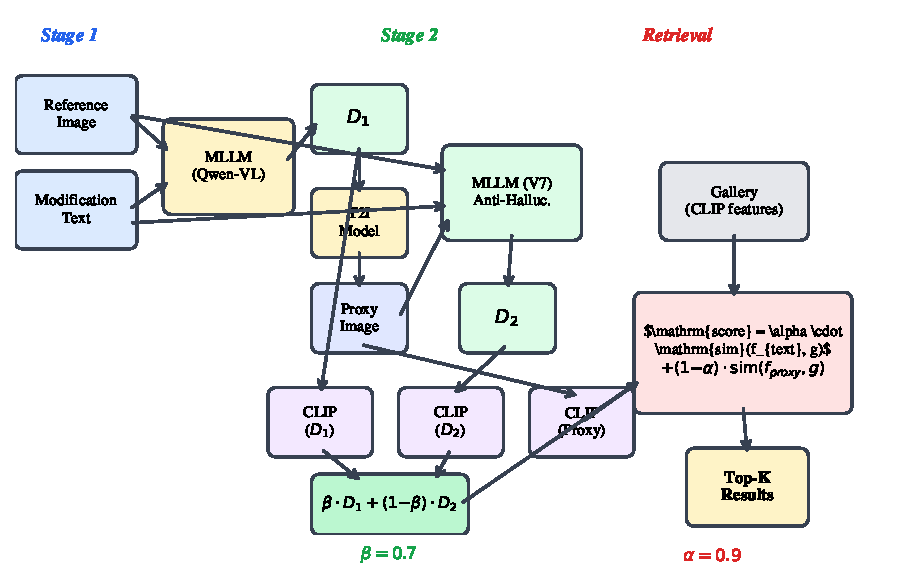
\includegraphics[width=0.92\textwidth]{fig_pipeline.pdf}
\vspace{0.3em}

\small
\textbf{三层创新}：
\begin{enumerate}\scriptsize
  \item \textcolor{tongjiBlue}{\textbf{视觉代理}}：$D_1 \to $ 文生图 $\to$ 代理图（提供图像空间信号）
  \item \textcolor{tongjiGreen}{\textbf{反幻觉精炼 (V7)}}：代理图只做诊断工具，不做描述来源
  \item \textcolor{tongjiRed}{\textbf{描述融合}}：$\beta \cdot \mathrm{CLIP}(D_1)+(1-\beta)\cdot \mathrm{CLIP}(D_2)$
\end{enumerate}
\end{frame}

\begin{frame}{\S2.1~创新点 1：视觉代理机制}
\textbf{核心思想}：把文本推理结果投射到图像空间，获得可视化的中间产物。

\vspace{0.5em}
\begin{columns}[T]
\begin{column}{0.48\textwidth}
\textbf{代理图的两类作用}：
\begin{itemize}\small
  \item \textbf{检索信号}：与文本特征互补，提供图像空间线索
  \item \textbf{诊断参照}：辅助第二轮判断 $D_1$ 是否准确表达修改意图
\end{itemize}

\vspace{0.5em}
\textbf{初步验证（FIQ dress 50 样本）}：
\begin{center}\small
\begin{tabular}{lc}
\toprule
方法 & R@10 \\
\midrule
Baseline (纯 $D_1$) & 18.0 \\
+ 后融合代理图 & \textbf{26.0} \up{8.0}\\
\bottomrule
\end{tabular}
\end{center}
\end{column}
\begin{column}{0.48\textwidth}
\textbf{实现细节}：
\begin{itemize}\small
  \item 文生图模型：MiniMax image-01
  \item 每条 $D_1$ 生成一张代理图
  \item 代理图用 CLIP ViT-L/14 编码
  \item 与 Gallery 图像在相同特征空间中计算相似度
\end{itemize}

\vspace{0.5em}
\begin{alertblock}{\small 关键挑战}
\small 代理图虽然有用，但 AI 生成\textbf{必然包含幻觉}，需要专门约束其使用方式。
\end{alertblock}
\end{column}
\end{columns}
\end{frame}

\begin{frame}{\S2.2~创新点 2：反幻觉 V7 提示词 (1/2)}
\textbf{核心矛盾}：代理图既是有用的参照，又是幻觉的来源。

\vspace{0.3em}
\textbf{Prompt 迭代历程（CIRR R@10, 200 样本）}：
\begin{center}
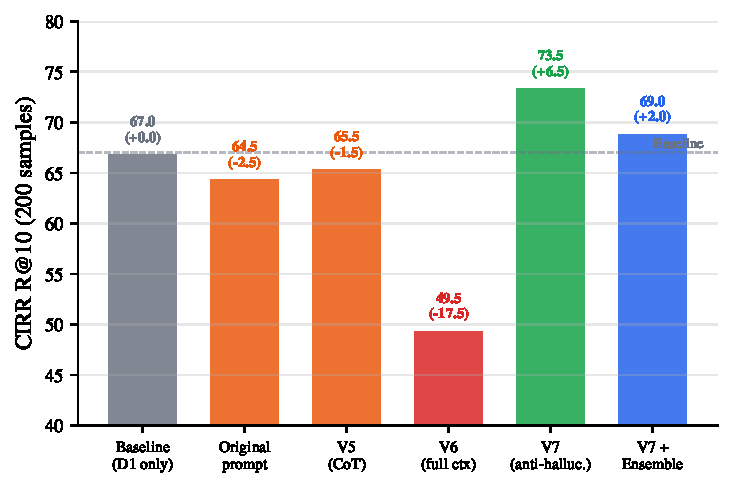
\includegraphics[width=0.72\textwidth]{fig_prompt_evolution.pdf}
\end{center}

\vspace{-0.2em}
\begin{itemize}\scriptsize
  \item[\xmark] \textbf{Original}：直接对比原图+代理图 $\to$ 描述膨胀 1.9倍，CIRR {\down{2.5}}
  \item[\xmark] \textbf{V5 (CoT)}：加入思维链结构 $\to$ 幻觉未解决，CIRR {\down{1.5}}
  \item[\xmark] \textbf{V6 (full ctx)}：传入完整 $D_1$ 上下文 $\to$ 信息过载，CIRR {\down{17.5}} \textbf{灾难性退化}
  \item[\cmark] \textbf{V7 (anti-hallucination)}：代理图仅做诊断 $\to$ CIRR {\up{6.5}} \textbf{关键突破}
\end{itemize}
\end{frame}

\begin{frame}[shrink=10]{\S2.2~反幻觉 V7 提示词 (2/2)}
\textbf{V7 核心设计}（3 条原则）：
\begin{enumerate}\footnotesize
  \item 明确告诉模型：\textit{``代理图是 AI 生成的，可能含有错误与幻觉''}
  \item 限定代理图唯一用途：\textbf{检查修改是否被正确应用}，不可复制其视觉细节
  \item 强制输出简短描述，只保留与检索最相关的核心属性
\end{enumerate}

\vspace{0.5em}
\textbf{任务范式的根本转变}：
\begin{center}\footnotesize
``重新描写目标图像''~$\Longrightarrow$~``在 $D_1$ 基础上做\textbf{最小必要修正}''
\end{center}

\vspace{0.5em}
\begin{block}{\footnotesize 核心洞察}
\footnotesize \textbf{信息过多反而有害}（V6 失败）；\textbf{限制信息来源比增加信息更重要}（V7 突破）。这是整个 prompt 工程中最关键的认识。
\end{block}
\end{frame}

\begin{frame}{\S2.3~创新点 3：描述融合与三路融合公式}
\textbf{问题}：V7 在 CIRR 上 {\up{6.5}}，但在 FIQ shirt 上 {\down{4.0}} —— 直接替换 $D_1$ 不稳定。

\vspace{0.8em}
\textbf{解决方案：CLIP 特征空间加权融合}（而非替换）

\begin{columns}[T]
\begin{column}{0.55\textwidth}
\begin{block}{文本融合公式}
\small
\[
\mathbf{f}_{\text{text}} = \mathrm{normalize}\big(\beta \cdot \mathrm{CLIP}(D_1) + (1-\beta) \cdot \mathrm{CLIP}(D_2)\big)
\]
\end{block}

\begin{block}{三路融合得分}
\small
\[
\mathrm{score}(I_c) = \alpha \cdot \mathrm{sim}(\mathbf{f}_{\text{text}}, \mathrm{CLIP}(I_c))
\]
\[
+ (1-\alpha) \cdot \mathrm{sim}(\mathrm{CLIP}(P), \mathrm{CLIP}(I_c))
\]
\end{block}
\end{column}
\begin{column}{0.42\textwidth}
\textbf{默认参数选择}：
\begin{itemize}\small
  \item $\beta = 0.7$：$D_1$ 占 70\%（兜底）+ $D_2$ 占 30\%（修正）
  \item $\alpha = 0.9$：文本占 90\%（主导）+ 代理图占 10\%（辅助）
\end{itemize}

\vspace{0.5em}
\textbf{设计哲学}：
\begin{center}\small
\textit{保守融合，稳中求进}\\
\textit{极端提升 $\Rightarrow$ 全局稳定}
\end{center}
\end{column}
\end{columns}

\vspace{0.3em}
\begin{center}\small
\textbf{效果}：V7+Ensemble 在 CIRR {\up{2.0}}、shirt {\up{0.5}}，\textbf{所有子集统一正向}。
\end{center}
\end{frame}

% ==================== Part 3: 实验结果 ====================
\section{实验结果}

\begin{frame}{\S3.1~实验设置}
\begin{columns}[T]
\begin{column}{0.55\textwidth}
\textbf{评估基准（9 个子任务）}：
\begin{itemize}\small
  \item \textbf{FashionIQ}：dress / shirt / toptee（服饰）
  \item \textbf{CIRCO}：开放域，123K 图库
  \item \textbf{CIRR}：自然场景，2297 图库
  \item \textbf{GeneCIS}：ch\_obj / fo\_obj / ch\_attr / fo\_attr（细粒度）
\end{itemize}

\vspace{0.5em}
\textbf{模型配置}：
\begin{itemize}\small
  \item MLLM：Qwen-VL-Max（替代原论文 GPT-4o）
  \item 文生图：MiniMax image-01
  \item 视觉编码：CLIP ViT-L/14（与原论文一致）
  \item 默认参数：$\beta=0.7$, $\alpha=0.9$
\end{itemize}
\end{column}
\begin{column}{0.42\textwidth}
\textbf{评估指标}：
\begin{itemize}\small
  \item FashionIQ / CIRR / GeneCIS：Recall@K
  \item CIRCO：mAP@K（多目标设置）
\end{itemize}

\vspace{0.5em}
\textbf{关于基线复现}：
\begin{itemize}\scriptsize
  \item 原论文 GPT-4o \textit{vs} 本文 Qwen-VL-Max
  \item FashionIQ dress R@10: 29.70 $\to$ 15.80
  \item \textbf{所有改进在同一基线上比较，公平}
\end{itemize}

\vspace{0.5em}
\textbf{花费}：MLLM + T2I API 约 \textbf{¥140}
\end{column}
\end{columns}
\end{frame}

\begin{frame}{\S3.2~主实验结果：9/9 数据集全部提升}
\begin{center}
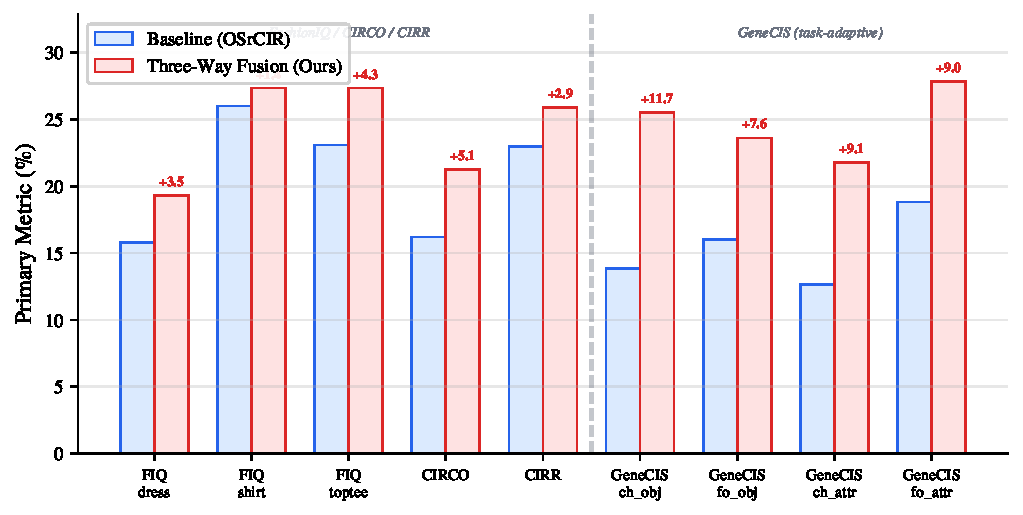
\includegraphics[width=0.92\textwidth]{fig_main_results.pdf}
\end{center}

\begin{center}\small
\textbf{35 项评估指标全部正向，0 退化}。左侧 5 个用默认参数，右侧 4 个 GeneCIS 用 task-adaptive 参数。
\end{center}
\end{frame}

\begin{frame}{\S3.3~主指标提升幅度}
\begin{columns}[T]
\begin{column}{0.48\textwidth}
\centering
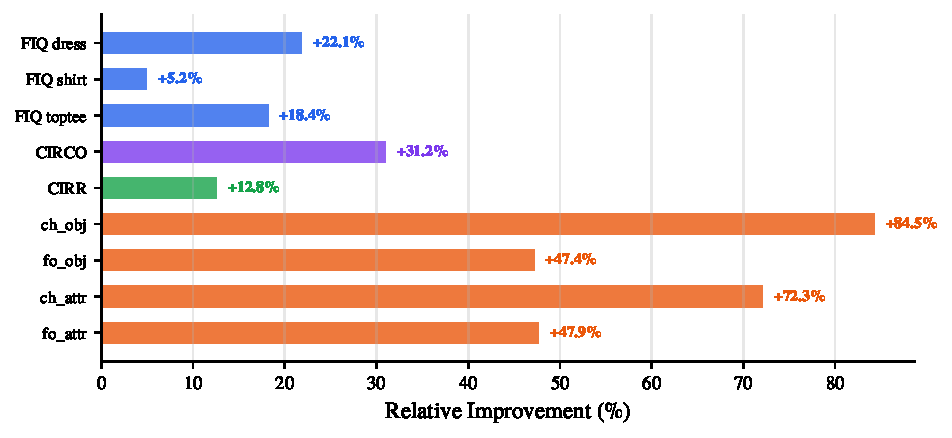
\includegraphics[width=\textwidth]{fig_relative.pdf}
\end{column}
\begin{column}{0.50\textwidth}
\scriptsize
\begin{tabular}{lccc}
\toprule
数据集 & Base. & Ours & 提升 \\
\midrule
FIQ dress & 15.80 & 19.29 & \up{22.1\%} \\
FIQ shirt & 26.00 & 27.35 & \up{5.2\%} \\
FIQ toptee & 23.09 & 27.35 & \up{18.4\%} \\
CIRCO & 16.21 & 21.26 & \up{31.2\%} \\
CIRR & 22.96 & 25.90 & \up{12.8\%} \\
\midrule
Gen ch\_obj & 13.83 & 25.51 & \up{84.5\%} \\
Gen fo\_obj & 16.02 & 23.62 & \up{47.4\%} \\
Gen ch\_attr & 12.65 & 21.79 & \up{72.3\%} \\
Gen fo\_attr & 18.82 & 27.83 & \up{47.9\%} \\
\bottomrule
\end{tabular}

\vspace{0.5em}
\footnotesize\textbf{亮点}：GeneCIS 最大 {\up{84.5\%}}；CIRCO {\up{31.2\%}}；FIQ shirt 最保守但仍 {\up{5.2\%}}
\end{column}
\end{columns}
\end{frame}

\begin{frame}{\S3.4~消融实验：$\alpha/\beta$ 参数敏感性分析}
\begin{center}
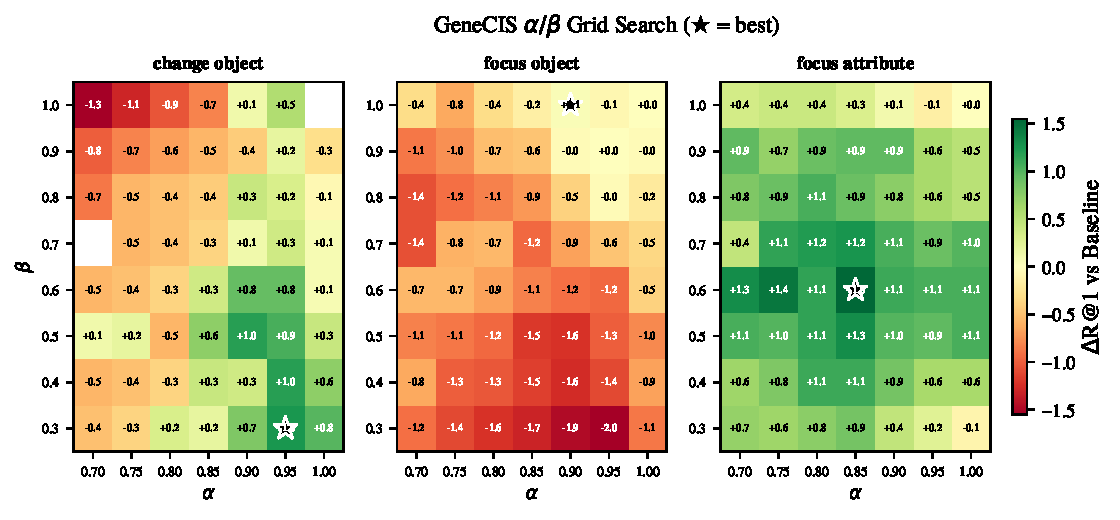
\includegraphics[width=\textwidth]{fig_heatmap.pdf}
\end{center}

\vspace{-0.2em}
\footnotesize\textbf{关键发现}：
\begin{itemize}\scriptsize
  \item \textbf{change\_object}：$\beta=0.3$（依赖 $D_2$）+ $\alpha=0.95$（弱代理图）
  \item \textbf{focus\_object}：$\beta=1.0$（完全不用 $D_2$！）\textendash\ V7 在短文本任务上 $D_2$ 退化为 1--3 词
  \item \textbf{focus\_attribute}：$\beta=0.6$ + $\alpha=0.85$（三路信号都发挥作用）
\end{itemize}
\textbf{结论}：不同任务对参数偏好截然不同，证明 \textbf{task-adaptive 参数} 是必要且有价值的。
\end{frame}

\begin{frame}{\S3.5~消融实验：模块贡献分析}
\begin{center}
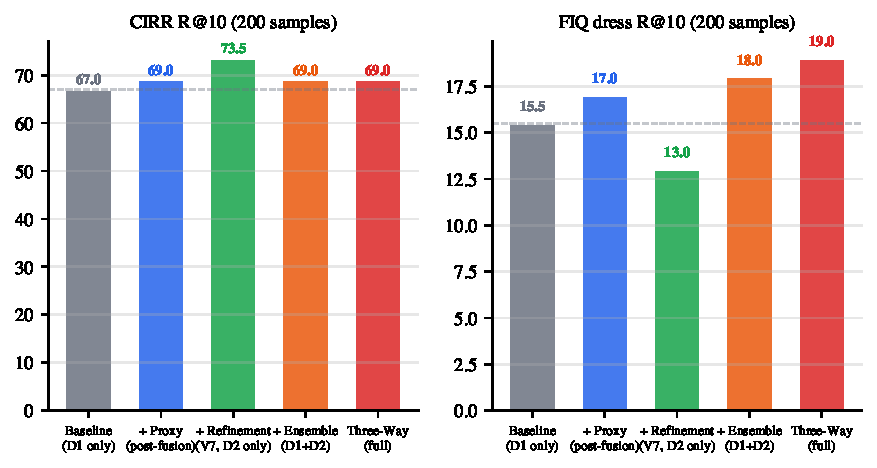
\includegraphics[width=0.9\textwidth]{fig_ablation.pdf}
\end{center}

\vspace{-0.3em}
\footnotesize\textbf{核心洞察}：不同数据集上模块最优配置\textbf{截然相反}
\begin{itemize}\scriptsize
  \item \textbf{CIRR}：V7 Refinement 是主力（{\up{6.5}}），Ensemble 会"拖累"
  \item \textbf{FIQ dress}：V7 反而退化（{\down{2.5}}），Ensemble 才是关键
  \item \textbf{三路融合的价值}：在同一框架下兼顾两端场景
\end{itemize}
\end{frame}

\begin{frame}[shrink=5]{\S3.6~FashionIQ 详细结果（12/12 正向）}
\begin{center}
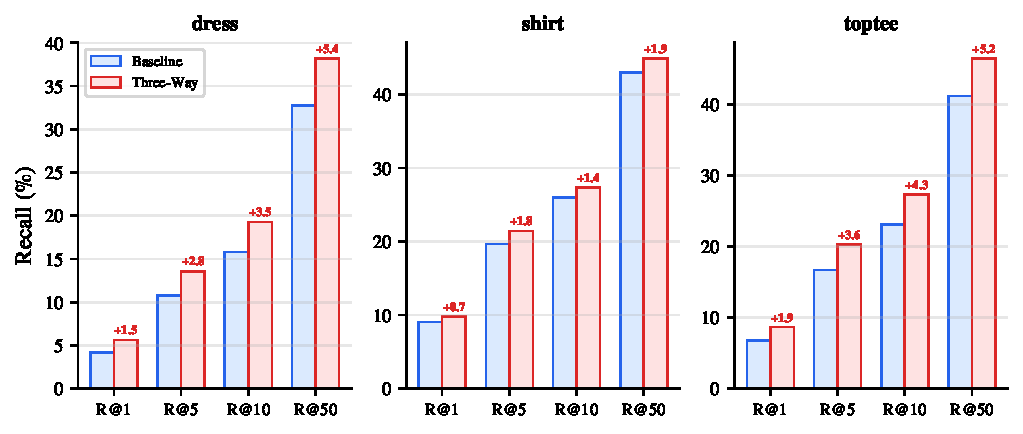
\includegraphics[width=0.95\textwidth]{fig_fashioniq.pdf}
\end{center}

\vspace{0.3em}
\scriptsize
\textbf{观察}：
\begin{itemize}\scriptsize
  \item \textbf{dress}：R@50 提升最大（{\up{5.4}}），颜色/款式变化敏感
  \item \textbf{shirt}：提升最保守（R@10 {\up{1.4}}），纹理细节难以捕获
  \item \textbf{toptee}：R@10 {\up{4.3}}，介于两者之间
\end{itemize}
\end{frame}

% ==================== Part 4: 总结 ====================
\section{总结与展望}

\begin{frame}[shrink=10]{\S4~工作总结}
\textbf{本文主要贡献}：
\begin{enumerate}\small
  \item[\cmark] 提出\textbf{视觉代理机制}：首次将文生图模型引入零样本组合检索，提供图像空间辅助信号
  \item[\cmark] 设计\textbf{V7 反幻觉提示词}：限定代理图的诊断角色，避免幻觉污染
  \item[\cmark] 构建\textbf{三路融合框架}：在 CLIP 空间统一三类信号，兼顾稳健性与性能
  \item[\cmark] 针对\textbf{GeneCIS 任务特性}提出专用 prompt + task-adaptive 参数
\end{enumerate}

\vspace{0.8em}
\textbf{实验验证}：
\begin{center}
\begin{tikzpicture}
\node[draw=tongjiRed, thick, rounded corners, fill=red!5, minimum width=11cm, minimum height=1.2cm] {
\large 9 个数据集 $\times$ 35 项指标 $=$ \textbf{\textcolor{tongjiRed}{35 项全部提升}}，\textbf{0 退化}
};
\end{tikzpicture}
\end{center}

\vspace{0.5em}
\begin{center}\small\textit{证明了在零样本组合检索中，\textbf{``多信号融合 + 幻觉约束''} 比``单点推理优化''更有价值。}
\end{center}
\end{frame}

\begin{frame}[shrink=5]{\S4~未来工作展望}
\begin{columns}[T]
\begin{column}{0.48\textwidth}
\textbf{短期改进方向}：
\begin{itemize}\small
  \item \textbf{自适应参数预测}：根据 query 特征动态选择 $\alpha/\beta$
  \item \textbf{多代理图策略}：生成多张代理图投票，减少单图噪声
  \item \textbf{更强 MLLM}：用 GPT-4o / Gemini 2.0 重新验证上限
\end{itemize}
\end{column}
\begin{column}{0.48\textwidth}
\textbf{长期扩展方向}：
\begin{itemize}\small
  \item \textbf{有监督 CIR}：迁移到训练数据充足场景
  \item \textbf{交互式检索}：支持多轮对话式精炼
  \item \textbf{视频组合检索}：扩展到时序维度
\end{itemize}
\end{column}
\end{columns}

\vspace{1.5em}
\begin{center}
\begin{tikzpicture}
\node[draw=tongjiBlue, thick, rounded corners, fill=blue!5, minimum width=10cm, minimum height=1.5cm, align=center] {
\Large\textbf{感谢各位老师！}\\
\small 欢迎批评指正
};
\end{tikzpicture}
\end{center}
\end{frame}

% ==================== 备用 Slide: 应对提问 ====================
\appendix

\begin{frame}[shrink=5]{附：关于 Baseline 差距的说明}
\scriptsize
\textbf{Q：本文 Baseline 远低于原论文报告值，结果是否可信？}

\vspace{0.3em}
\textbf{原因分析}：
\begin{itemize}\scriptsize
  \item 原论文使用 GPT-4o，本文因 API 可用性改用 Qwen-VL-Max
  \item Qwen-VL-Max 在服饰细粒度描述上不及 GPT-4o（FashionIQ 差约 14pp）
  \item 但 GeneCIS focus\_object 上 Qwen-VL 反而略胜 GPT-4o（16.02 vs 15.00）
\end{itemize}

\vspace{0.3em}
\textbf{对公平性的影响：无}
\begin{itemize}\scriptsize
  \item 所有改进均在\textbf{同一 Baseline} 上对比，相对提升可比
  \item 使用 Qwen-VL-Max 只降低绝对值，不改变方法有效性
  \item 三路融合的核心逻辑（代理 + 反幻觉 + 融合）是模型无关的
\end{itemize}
\end{frame}

\begin{frame}{附：关于参数选择的说明}
\scriptsize
\textbf{Q：为什么选 $\beta=0.7$、$\alpha=0.9$？是否经过调优？}

\vspace{0.3em}
\textbf{$\beta=0.7$ 的依据}：
\begin{itemize}\scriptsize
  \item $D_1$ 信息完整度 > $D_2$（V7 prompt 要求简短）
  \item 若 $\beta < 0.5$，FIQ shirt 会因 $D_2$ 过激精炼而退化
  \item FashionIQ + CIRR 联合调参的折中点
\end{itemize}

\vspace{0.3em}
\textbf{$\alpha=0.9$ 的依据}：
\begin{itemize}\scriptsize
  \item 代理图含 AI 幻觉，不宜主导检索（$\alpha < 0.5$ 时 CIRCO 明显退化）
  \item 10\% 权重足以提供互补信号，不导致场景偏移
\end{itemize}

\vspace{0.3em}
\textbf{GeneCIS 为何需要 task-adaptive}：
\begin{itemize}\scriptsize
  \item 修改文本仅 1--2 词，V7 的``描述不超过修改文本''限制使 $D_2$ 退化
  \item 每个 query 仅 $\sim$14 张候选图，代理图场景偏好影响被放大
  \item 网格搜索：各子集最优参数 $\beta$ 从 0.3 到 1.0，差异显著
\end{itemize}
\end{frame}

\end{document}
